\documentclass[12pt,]{article}
\usepackage{lmodern}
\usepackage{amssymb,amsmath}
\usepackage{ifxetex,ifluatex}
\usepackage{fixltx2e} % provides \textsubscript
\ifnum 0\ifxetex 1\fi\ifluatex 1\fi=0 % if pdftex
  \usepackage[T1]{fontenc}
  \usepackage[utf8]{inputenc}
\else % if luatex or xelatex
  \ifxetex
    \usepackage{mathspec}
  \else
    \usepackage{fontspec}
  \fi
  \defaultfontfeatures{Ligatures=TeX,Scale=MatchLowercase}
\fi
% use upquote if available, for straight quotes in verbatim environments
\IfFileExists{upquote.sty}{\usepackage{upquote}}{}
% use microtype if available
\IfFileExists{microtype.sty}{%
\usepackage{microtype}
\UseMicrotypeSet[protrusion]{basicmath} % disable protrusion for tt fonts
}{}
\usepackage[margin = 1.5in]{geometry}
\usepackage{hyperref}
\PassOptionsToPackage{usenames,dvipsnames}{color} % color is loaded by hyperref
\hypersetup{unicode=true,
            pdftitle={More Tips and Tricks},
            pdfauthor={Abhinav Anand, IIMB},
            colorlinks=true,
            linkcolor=blue,
            citecolor=magenta,
            urlcolor=red,
            breaklinks=true}
\urlstyle{same}  % don't use monospace font for urls
\usepackage{color}
\usepackage{fancyvrb}
\newcommand{\VerbBar}{|}
\newcommand{\VERB}{\Verb[commandchars=\\\{\}]}
\DefineVerbatimEnvironment{Highlighting}{Verbatim}{commandchars=\\\{\}}
% Add ',fontsize=\small' for more characters per line
\usepackage{framed}
\definecolor{shadecolor}{RGB}{248,248,248}
\newenvironment{Shaded}{\begin{snugshade}}{\end{snugshade}}
\newcommand{\KeywordTok}[1]{\textcolor[rgb]{0.13,0.29,0.53}{\textbf{#1}}}
\newcommand{\DataTypeTok}[1]{\textcolor[rgb]{0.13,0.29,0.53}{#1}}
\newcommand{\DecValTok}[1]{\textcolor[rgb]{0.00,0.00,0.81}{#1}}
\newcommand{\BaseNTok}[1]{\textcolor[rgb]{0.00,0.00,0.81}{#1}}
\newcommand{\FloatTok}[1]{\textcolor[rgb]{0.00,0.00,0.81}{#1}}
\newcommand{\ConstantTok}[1]{\textcolor[rgb]{0.00,0.00,0.00}{#1}}
\newcommand{\CharTok}[1]{\textcolor[rgb]{0.31,0.60,0.02}{#1}}
\newcommand{\SpecialCharTok}[1]{\textcolor[rgb]{0.00,0.00,0.00}{#1}}
\newcommand{\StringTok}[1]{\textcolor[rgb]{0.31,0.60,0.02}{#1}}
\newcommand{\VerbatimStringTok}[1]{\textcolor[rgb]{0.31,0.60,0.02}{#1}}
\newcommand{\SpecialStringTok}[1]{\textcolor[rgb]{0.31,0.60,0.02}{#1}}
\newcommand{\ImportTok}[1]{#1}
\newcommand{\CommentTok}[1]{\textcolor[rgb]{0.56,0.35,0.01}{\textit{#1}}}
\newcommand{\DocumentationTok}[1]{\textcolor[rgb]{0.56,0.35,0.01}{\textbf{\textit{#1}}}}
\newcommand{\AnnotationTok}[1]{\textcolor[rgb]{0.56,0.35,0.01}{\textbf{\textit{#1}}}}
\newcommand{\CommentVarTok}[1]{\textcolor[rgb]{0.56,0.35,0.01}{\textbf{\textit{#1}}}}
\newcommand{\OtherTok}[1]{\textcolor[rgb]{0.56,0.35,0.01}{#1}}
\newcommand{\FunctionTok}[1]{\textcolor[rgb]{0.00,0.00,0.00}{#1}}
\newcommand{\VariableTok}[1]{\textcolor[rgb]{0.00,0.00,0.00}{#1}}
\newcommand{\ControlFlowTok}[1]{\textcolor[rgb]{0.13,0.29,0.53}{\textbf{#1}}}
\newcommand{\OperatorTok}[1]{\textcolor[rgb]{0.81,0.36,0.00}{\textbf{#1}}}
\newcommand{\BuiltInTok}[1]{#1}
\newcommand{\ExtensionTok}[1]{#1}
\newcommand{\PreprocessorTok}[1]{\textcolor[rgb]{0.56,0.35,0.01}{\textit{#1}}}
\newcommand{\AttributeTok}[1]{\textcolor[rgb]{0.77,0.63,0.00}{#1}}
\newcommand{\RegionMarkerTok}[1]{#1}
\newcommand{\InformationTok}[1]{\textcolor[rgb]{0.56,0.35,0.01}{\textbf{\textit{#1}}}}
\newcommand{\WarningTok}[1]{\textcolor[rgb]{0.56,0.35,0.01}{\textbf{\textit{#1}}}}
\newcommand{\AlertTok}[1]{\textcolor[rgb]{0.94,0.16,0.16}{#1}}
\newcommand{\ErrorTok}[1]{\textcolor[rgb]{0.64,0.00,0.00}{\textbf{#1}}}
\newcommand{\NormalTok}[1]{#1}
\usepackage{graphicx,grffile}
\makeatletter
\def\maxwidth{\ifdim\Gin@nat@width>\linewidth\linewidth\else\Gin@nat@width\fi}
\def\maxheight{\ifdim\Gin@nat@height>\textheight\textheight\else\Gin@nat@height\fi}
\makeatother
% Scale images if necessary, so that they will not overflow the page
% margins by default, and it is still possible to overwrite the defaults
% using explicit options in \includegraphics[width, height, ...]{}
\setkeys{Gin}{width=\maxwidth,height=\maxheight,keepaspectratio}
\IfFileExists{parskip.sty}{%
\usepackage{parskip}
}{% else
\setlength{\parindent}{0pt}
\setlength{\parskip}{6pt plus 2pt minus 1pt}
}
\setlength{\emergencystretch}{3em}  % prevent overfull lines
\providecommand{\tightlist}{%
  \setlength{\itemsep}{0pt}\setlength{\parskip}{0pt}}
\setcounter{secnumdepth}{0}
% Redefines (sub)paragraphs to behave more like sections
\ifx\paragraph\undefined\else
\let\oldparagraph\paragraph
\renewcommand{\paragraph}[1]{\oldparagraph{#1}\mbox{}}
\fi
\ifx\subparagraph\undefined\else
\let\oldsubparagraph\subparagraph
\renewcommand{\subparagraph}[1]{\oldsubparagraph{#1}\mbox{}}
\fi

%%% Use protect on footnotes to avoid problems with footnotes in titles
\let\rmarkdownfootnote\footnote%
\def\footnote{\protect\rmarkdownfootnote}

%%% Change title format to be more compact
\usepackage{titling}

% Create subtitle command for use in maketitle
\providecommand{\subtitle}[1]{
  \posttitle{
    \begin{center}\large#1\end{center}
    }
}

\setlength{\droptitle}{-2em}

  \title{More Tips and Tricks}
    \pretitle{\vspace{\droptitle}\centering\huge}
  \posttitle{\par}
    \author{Abhinav Anand, IIMB}
    \preauthor{\centering\large\emph}
  \postauthor{\par}
      \predate{\centering\large\emph}
  \postdate{\par}
    \date{2019/06/18}

\linespread{1.3}

\begin{document}
\maketitle

\section{Scripts in R}\label{scripts-in-r}

Scripts are files (ending in \texttt{.R}) that contain sequences of
instructions that we can command a machine to follow. Consier a typical
empirical project: we need to read data stored in some type of file;
then clean and tidy it, then process it and use descriptive statistics
and plots to delineate its features etc. All this can be achieved by
storing a sequence of instructions in a script file. Data can be read
using the the \texttt{read\_csv()} function, processing can be done
using the package \texttt{dplyr} etc.

\section{Linear regression in R}\label{linear-regression-in-r}

Generally a linear model takes the following form:

\[
y = \beta_0 + \beta_1x_1 + \hdots + \beta_mx_m + u
\] where \(u_{n\times 1}\) is the error term. This setup corresponds to
an overdetermined linear system of equations leading to a least squares
solution:

\[
\hat{\beta} = (X^{\top} X)^{-1} X^{\top}y 
\]

where the explanatory matrix \(X_{m\times n}\) contains independent
variables \(x_1,\hdots,x_m\) as column vectors of size \(n\times 1\).

One of the strengths of R is the flexibility and support it offers for
linear regression modeling. In order to illustrate it more fully, let us
consider data for India in the \texttt{gapminder} dataset.

\begin{Shaded}
\begin{Highlighting}[]
\NormalTok{data_Ind <-}\StringTok{ }\NormalTok{gapminder}\OperatorTok{::}\NormalTok{gapminder }\OperatorTok\StringTok{ }
\StringTok{  }\NormalTok{dplyr}\OperatorTok{::}\KeywordTok{filter}\NormalTok{(country }\OperatorTok{==}\StringTok{ "India"}\NormalTok{)}

\KeywordTok{ggplot}\NormalTok{(data_Ind, }\KeywordTok{aes}\NormalTok{(year, gdpPercap)) }\OperatorTok{+}
\StringTok{  }\KeywordTok{geom_point}\NormalTok{() }\OperatorTok{+}
\StringTok{  }\KeywordTok{geom_line}\NormalTok{() }
\end{Highlighting}
\end{Shaded}

\begin{center}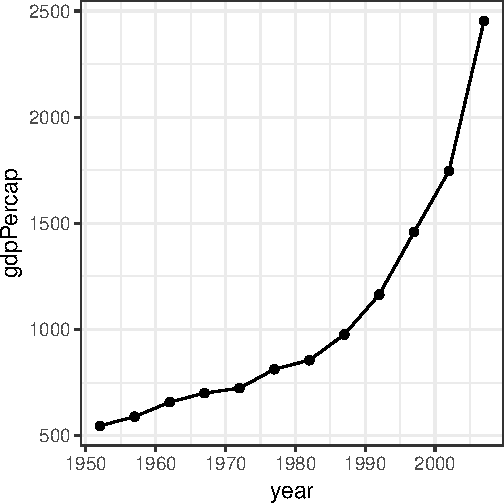
\includegraphics{Intro_tips_tricks_files/figure-latex/data_Ind_GDP-1} \end{center}

We see that there has been a large increase in GDP per capita in India.
A similar trend is observed for life expectancy:

\begin{Shaded}
\begin{Highlighting}[]
\KeywordTok{ggplot}\NormalTok{(data_Ind, }\KeywordTok{aes}\NormalTok{(year, lifeExp)) }\OperatorTok{+}
\StringTok{  }\KeywordTok{geom_point}\NormalTok{() }\OperatorTok{+}
\StringTok{  }\KeywordTok{geom_line}\NormalTok{() }
\end{Highlighting}
\end{Shaded}

\begin{center}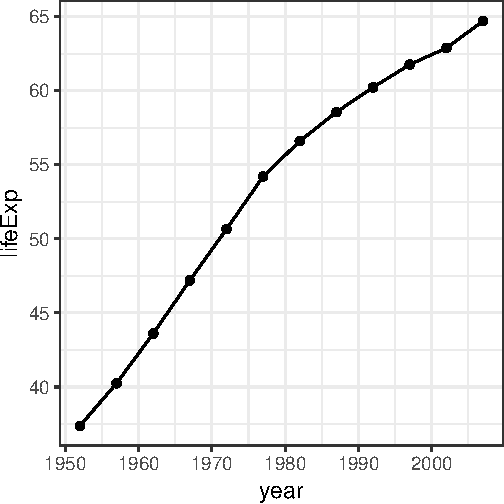
\includegraphics{Intro_tips_tricks_files/figure-latex/data_Ind_lifeexp-1} \end{center}

What about the relationship between the two? For example, (all else
equal) does GDP per capita of India explain the life expectancy trends
observed?

\begin{Shaded}
\begin{Highlighting}[]
\KeywordTok{ggplot}\NormalTok{(data_Ind, }\KeywordTok{aes}\NormalTok{(gdpPercap, lifeExp)) }\OperatorTok{+}
\StringTok{  }\KeywordTok{geom_point}\NormalTok{() }
\end{Highlighting}
\end{Shaded}

\begin{center}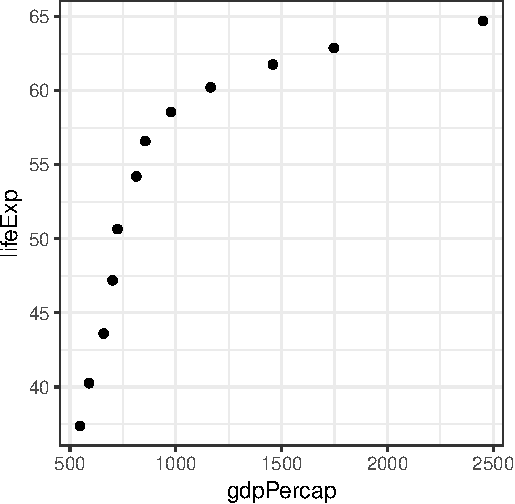
\includegraphics{Intro_tips_tricks_files/figure-latex/data_Ind_scatter-1} \end{center}

This suggests that the two variables share a positive relation. We can
try to check this by means of a linear regression in the following way:

\[
\text{life exp} = \beta_0 + \beta_1 \text{(gdp percap)} + u
\]

In order to implement this step in R is via the following:

\begin{Shaded}
\begin{Highlighting}[]
\NormalTok{lm_formula <-}\StringTok{ }\NormalTok{lifeExp }\OperatorTok{~}\StringTok{ }\NormalTok{gdpPercap}

\NormalTok{lm_life_gdppc <-}\StringTok{ }\KeywordTok{lm}\NormalTok{(}\DataTypeTok{data =}\NormalTok{ data_Ind, }\DataTypeTok{formula =}\NormalTok{ lm_formula)}

\KeywordTok{summary}\NormalTok{(lm_life_gdppc)}
\end{Highlighting}
\end{Shaded}

\begin{verbatim}
## 
## Call:
## lm(formula = lm_formula, data = data_Ind)
## 
## Residuals:
##    Min     1Q Median     3Q    Max 
## -9.155 -4.931  1.284  4.576  6.437 
## 
## Coefficients:
##              Estimate Std. Error t value Pr(>|t|)    
## (Intercept) 39.423336   3.659432  10.773    8e-07 ***
## gdpPercap    0.012998   0.003075   4.227  0.00175 ** 
## ---
## Signif. codes:  0 '***' 0.001 '**' 0.01 '*' 0.05 '.' 0.1 ' ' 1
## 
## Residual standard error: 5.816 on 10 degrees of freedom
## Multiple R-squared:  0.6411, Adjusted R-squared:  0.6052 
## F-statistic: 17.86 on 1 and 10 DF,  p-value: 0.001753
\end{verbatim}

\begin{Shaded}
\begin{Highlighting}[]
\KeywordTok{ggplot}\NormalTok{(data_Ind, }\KeywordTok{aes}\NormalTok{(gdpPercap, lifeExp)) }\OperatorTok{+}
\StringTok{  }\KeywordTok{geom_point}\NormalTok{() }\OperatorTok{+}
\StringTok{  }\KeywordTok{geom_smooth}\NormalTok{(}\DataTypeTok{method =} \StringTok{"lm"}\NormalTok{)}
\end{Highlighting}
\end{Shaded}

\begin{center}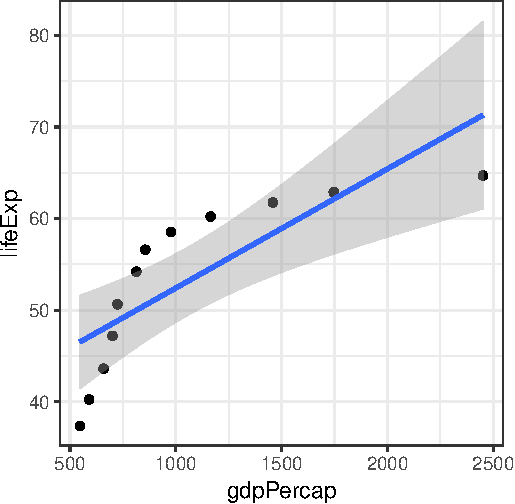
\includegraphics{Intro_tips_tricks_files/figure-latex/data_Ind_lm-1} \end{center}

What is this object \texttt{lm\_life\_gdppc}? What is its structure? We
can quickly check by accessing its contents:

\begin{Shaded}
\begin{Highlighting}[]
\KeywordTok{names}\NormalTok{(lm_life_gdppc)}
\end{Highlighting}
\end{Shaded}

\begin{verbatim}
##  [1] "coefficients"  "residuals"     "effects"       "rank"         
##  [5] "fitted.values" "assign"        "qr"            "df.residual"  
##  [9] "xlevels"       "call"          "terms"         "model"
\end{verbatim}

What about some subset of data, say the period before 1990?

\begin{Shaded}
\begin{Highlighting}[]
\KeywordTok{lm}\NormalTok{(}\KeywordTok{filter}\NormalTok{(data_Ind, year }\OperatorTok{<=}\StringTok{ }\DecValTok{1990}\NormalTok{), }\DataTypeTok{formula =}\NormalTok{ lm_formula) }\OperatorTok\StringTok{ }
\StringTok{  }\KeywordTok{summary}\NormalTok{()}
\end{Highlighting}
\end{Shaded}

\begin{verbatim}
## 
## Call:
## lm(formula = lm_formula, data = filter(data_Ind, year <= 1990))
## 
## Residuals:
##     Min      1Q  Median      3Q     Max 
## -2.8626 -1.0747 -0.1943  1.4541  2.5804 
## 
## Coefficients:
##             Estimate Std. Error t value Pr(>|t|)    
## (Intercept)  9.80149    3.83775   2.554   0.0433 *  
## gdpPercap    0.05286    0.00515  10.264 4.99e-05 ***
## ---
## Signif. codes:  0 '***' 0.001 '**' 0.01 '*' 0.05 '.' 0.1 ' ' 1
## 
## Residual standard error: 1.945 on 6 degrees of freedom
## Multiple R-squared:  0.9461, Adjusted R-squared:  0.9371 
## F-statistic: 105.3 on 1 and 6 DF,  p-value: 4.992e-05
\end{verbatim}

\begin{Shaded}
\begin{Highlighting}[]
\KeywordTok{ggplot}\NormalTok{(}\KeywordTok{filter}\NormalTok{(data_Ind, year }\OperatorTok{<=}\StringTok{ }\DecValTok{1990}\NormalTok{), }\KeywordTok{aes}\NormalTok{(lifeExp, gdpPercap)) }\OperatorTok{+}
\StringTok{  }\KeywordTok{geom_point}\NormalTok{() }\OperatorTok{+}
\StringTok{  }\KeywordTok{geom_smooth}\NormalTok{(}\DataTypeTok{method =} \StringTok{"lm"}\NormalTok{)}
\end{Highlighting}
\end{Shaded}

\begin{center}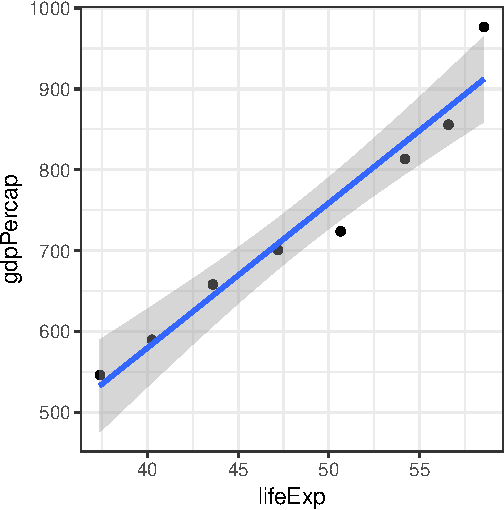
\includegraphics{Intro_tips_tricks_files/figure-latex/data_Ind_lm_subset-1} \end{center}

\subsection{Nonlinear relationships}\label{nonlinear-relationships}

The plot between the dependent and independent variable suggest a
nonlinear relationship. Can we test this simply? Let's consider the
following modification:

\[
\text{life exp} = \beta_0 + \beta_1 \text{(gdp percap)}^2 + u
\]

In general, R can accommodate independent variables involving
mathematical operators in a regression equation with the function
\texttt{I()}.

\begin{Shaded}
\begin{Highlighting}[]
\NormalTok{lm_formula_quad <-}\StringTok{ }\NormalTok{lifeExp }\OperatorTok{~}\StringTok{ }\KeywordTok{I}\NormalTok{(gdpPercap)}\OperatorTok{^}\DecValTok{2}

\NormalTok{lm_life_gdppc_quad <-}\StringTok{ }\KeywordTok{lm}\NormalTok{(}\DataTypeTok{data =}\NormalTok{ data_Ind, }\DataTypeTok{formula =}\NormalTok{ lm_formula_quad)}

\KeywordTok{summary}\NormalTok{(lm_life_gdppc_quad)}
\end{Highlighting}
\end{Shaded}

\begin{verbatim}
## 
## Call:
## lm(formula = lm_formula_quad, data = data_Ind)
## 
## Residuals:
##    Min     1Q Median     3Q    Max 
## -9.155 -4.931  1.284  4.576  6.437 
## 
## Coefficients:
##               Estimate Std. Error t value Pr(>|t|)    
## (Intercept)  39.423336   3.659432  10.773    8e-07 ***
## I(gdpPercap)  0.012998   0.003075   4.227  0.00175 ** 
## ---
## Signif. codes:  0 '***' 0.001 '**' 0.01 '*' 0.05 '.' 0.1 ' ' 1
## 
## Residual standard error: 5.816 on 10 degrees of freedom
## Multiple R-squared:  0.6411, Adjusted R-squared:  0.6052 
## F-statistic: 17.86 on 1 and 10 DF,  p-value: 0.001753
\end{verbatim}

\begin{Shaded}
\begin{Highlighting}[]
\KeywordTok{ggplot}\NormalTok{(data_Ind, }\KeywordTok{aes}\NormalTok{(}\DataTypeTok{x =}\NormalTok{ gdpPercap, }\DataTypeTok{y =}\NormalTok{ lifeExp)) }\OperatorTok{+}
\StringTok{  }\KeywordTok{geom_point}\NormalTok{() }\OperatorTok{+}
\StringTok{  }\KeywordTok{stat_smooth}\NormalTok{(}\DataTypeTok{method =} \StringTok{"lm"}\NormalTok{, }
              \DataTypeTok{formula =}\NormalTok{ y }\OperatorTok{~}\StringTok{ }\KeywordTok{poly}\NormalTok{(x, }\DecValTok{2}\NormalTok{), }\CommentTok{#polynomial order 2}
              \DataTypeTok{size =} \FloatTok{0.8}\NormalTok{,}
              \DataTypeTok{linetype =} \StringTok{"dashed"}
\NormalTok{              )}
\end{Highlighting}
\end{Shaded}

\begin{center}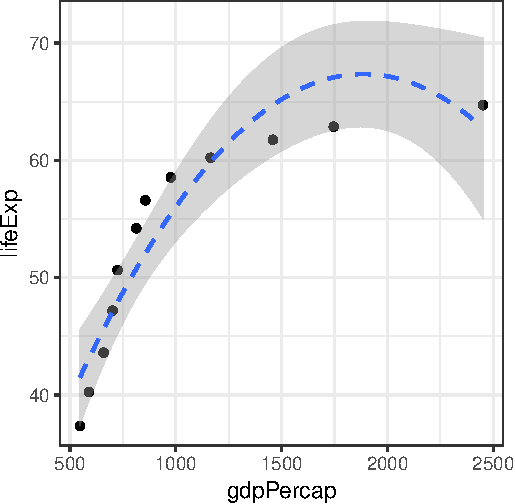
\includegraphics{Intro_tips_tricks_files/figure-latex/data_Ind_lm_quad-1} \end{center}

\begin{Shaded}
\begin{Highlighting}[]
\CommentTok{# What about higher order polynomials?}
\KeywordTok{ggplot}\NormalTok{(data_Ind, }\KeywordTok{aes}\NormalTok{(}\DataTypeTok{x =}\NormalTok{ gdpPercap, }\DataTypeTok{y =}\NormalTok{ lifeExp)) }\OperatorTok{+}
\StringTok{  }\KeywordTok{geom_point}\NormalTok{() }\OperatorTok{+}
\StringTok{  }\KeywordTok{stat_smooth}\NormalTok{(}\DataTypeTok{method =} \StringTok{"lm"}\NormalTok{, }
              \DataTypeTok{formula =}\NormalTok{ y }\OperatorTok{~}\StringTok{ }\KeywordTok{poly}\NormalTok{(x, }\DecValTok{3}\NormalTok{), }\CommentTok{#polynomial order 3}
              \DataTypeTok{size =} \FloatTok{0.8}\NormalTok{,}
              \DataTypeTok{linetype =} \StringTok{"dotdash"}
\NormalTok{              )}
\end{Highlighting}
\end{Shaded}

\begin{center}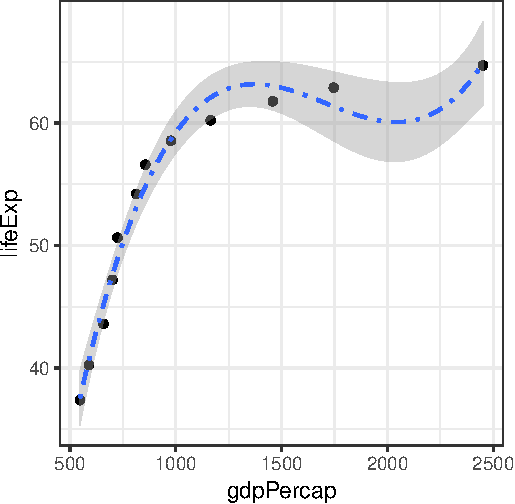
\includegraphics{Intro_tips_tricks_files/figure-latex/data_Ind_lm_quad-2} \end{center}

Are visually better fits also evidence of better underlying models? This
is a hard question to answer in general---all else equal we prefer
models that are parsimonious (have fewer explanatory variables).

\section{Functional Programming in R}\label{functional-programming-in-r}

Another very powerful feature of R is its support for functional
programming, which in general, involves applying functions to arrays,
dataframes, lists etc.

For example, how should one compute the mean across rows of a matrix?

\begin{Shaded}
\begin{Highlighting}[]
\NormalTok{df <-}\StringTok{ }\KeywordTok{data.frame}\NormalTok{(}\DataTypeTok{C_1 =} \KeywordTok{rnorm}\NormalTok{(}\DecValTok{10}\NormalTok{, }\DecValTok{0}\NormalTok{, }\DecValTok{1}\NormalTok{), }
                 \DataTypeTok{C_2 =} \KeywordTok{rnorm}\NormalTok{(}\DecValTok{10}\NormalTok{, }\DecValTok{1}\NormalTok{, }\DecValTok{2}\NormalTok{),}
                 \DataTypeTok{C_3 =} \KeywordTok{rnorm}\NormalTok{(}\DecValTok{10}\NormalTok{, }\DecValTok{2}\NormalTok{, }\DecValTok{3}\NormalTok{)}
\NormalTok{                 )}

\KeywordTok{head}\NormalTok{(df)}
\end{Highlighting}
\end{Shaded}

\begin{verbatim}
##           C_1         C_2        C_3
## 1 -0.09280755  3.16525877 -0.1326818
## 2 -1.72400687  0.70561317  9.2879545
## 3 -0.87588162  0.09011416  6.6904262
## 4 -0.49597151 -0.15796488 -1.1483896
## 5 -1.76524218 -0.13320632  2.1716311
## 6 -1.01364069 -0.53340528  2.0441538
\end{verbatim}

\begin{Shaded}
\begin{Highlighting}[]
\CommentTok{# One way to solve the problem}
\NormalTok{rmean_}\DecValTok{1}\NormalTok{ <-}\StringTok{ }\KeywordTok{rowMeans}\NormalTok{(df)}
\KeywordTok{print}\NormalTok{(rmean_}\DecValTok{1}\NormalTok{)}
\end{Highlighting}
\end{Shaded}

\begin{verbatim}
##  [1]  0.97992314  2.75652025  1.96821958 -0.60077534  0.09106087
##  [6]  0.16570260  1.17545975 -1.24629421  1.78506284  0.58475120
\end{verbatim}

\begin{Shaded}
\begin{Highlighting}[]
\CommentTok{# Another more 'functional' way}
\NormalTok{func_mean <-}\StringTok{ }\ControlFlowTok{function}\NormalTok{(vec)}
\NormalTok{\{}
  \KeywordTok{return}\NormalTok{(}\KeywordTok{mean}\NormalTok{(vec, }\DataTypeTok{na.rm =}\NormalTok{ T))}
\NormalTok{\}}

\CommentTok{# Apply function on rows}
\NormalTok{rmean_}\DecValTok{2}\NormalTok{ <-}\StringTok{ }\KeywordTok{apply}\NormalTok{(df, }\DecValTok{1}\NormalTok{, func_mean) }
\KeywordTok{print}\NormalTok{(rmean_}\DecValTok{1}\NormalTok{)}
\end{Highlighting}
\end{Shaded}

\begin{verbatim}
##  [1]  0.97992314  2.75652025  1.96821958 -0.60077534  0.09106087
##  [6]  0.16570260  1.17545975 -1.24629421  1.78506284  0.58475120
\end{verbatim}

\begin{Shaded}
\begin{Highlighting}[]
\CommentTok{# Apply function on columns}
\NormalTok{rmean_}\DecValTok{3}\NormalTok{ <-}\StringTok{ }\KeywordTok{apply}\NormalTok{(df, }\DecValTok{2}\NormalTok{, func_mean)}
\KeywordTok{print}\NormalTok{(rmean_}\DecValTok{3}\NormalTok{)}
\end{Highlighting}
\end{Shaded}

\begin{verbatim}
##        C_1        C_2        C_3 
## -0.1797416  0.7129948  1.7646360
\end{verbatim}

Note how to use the \texttt{apply()} function. We \texttt{apply()} the
function over rows or columns or other dimensions. In general that's the
philosophy of the \texttt{apply()} family of functions, which includes
functions \texttt{lapply()} (list-apply) and \texttt{sapply()}
(simplify-apply) etc. The function \texttt{lapply} returns a list and
\texttt{sapply} a vector (if possible). In both cases the first argument
is a list (or dataframe) and the second argument is the name of a
function.

What is a list? It's essentially a more general version of a dataframe
and can contain not only dissimilar data types but also, say dataframes
within them.

\begin{Shaded}
\begin{Highlighting}[]
\NormalTok{temp_list <-}\StringTok{ }\KeywordTok{list}\NormalTok{(}\DataTypeTok{a =} \KeywordTok{runif}\NormalTok{(}\DecValTok{10}\NormalTok{),}
                  \DataTypeTok{b =} \StringTok{"Happy birthday"}\NormalTok{,}
                  \DataTypeTok{c =} \KeywordTok{data.frame}\NormalTok{(}\DataTypeTok{x =} \KeywordTok{rnorm}\NormalTok{(}\DecValTok{10}\NormalTok{, }\DecValTok{0}\NormalTok{, }\DecValTok{1}\NormalTok{)),}
                  \DataTypeTok{d =} \KeywordTok{sample}\NormalTok{(letters, }\DecValTok{7}\NormalTok{, }\DataTypeTok{replace =} \OtherTok{TRUE}\NormalTok{)}
\NormalTok{                  )}
\KeywordTok{str}\NormalTok{(temp_list) }\CommentTok{#structure of the list}
\end{Highlighting}
\end{Shaded}

\begin{verbatim}
## List of 4
##  $ a: num [1:10] 0.492 0.989 0.412 0.559 0.126 ...
##  $ b: chr "Happy birthday"
##  $ c:'data.frame':   10 obs. of  1 variable:
##   ..$ x: num [1:10] 2.559 1.171 0.301 -0.915 -1 ...
##  $ d: chr [1:7] "p" "t" "o" "n" ...
\end{verbatim}

\begin{Shaded}
\begin{Highlighting}[]
\CommentTok{# 1apply() is used to apply the same function to each}
\CommentTok{# "cell" of the list}
\KeywordTok{lapply}\NormalTok{(temp_list, is.numeric) }\CommentTok{#check if each cell is numeric}
\end{Highlighting}
\end{Shaded}

\begin{verbatim}
## $a
## [1] TRUE
## 
## $b
## [1] FALSE
## 
## $c
## [1] FALSE
## 
## $d
## [1] FALSE
\end{verbatim}

\begin{Shaded}
\begin{Highlighting}[]
\CommentTok{# contrast with sapply()}
\KeywordTok{sapply}\NormalTok{(temp_list, is.numeric)}
\end{Highlighting}
\end{Shaded}

\begin{verbatim}
##     a     b     c     d 
##  TRUE FALSE FALSE FALSE
\end{verbatim}

\subsection{\texorpdfstring{The \texttt{map()} family from
\texttt{purrr}}{The map() family from purrr}}\label{the-map-family-from-purrr}

The \texttt{map} function does the exact same operation as
\texttt{apply} but is consistent with the output format type. For
example \texttt{map()} returns a list, \texttt{map\_dbl()} returns a
double type vector, \texttt{map\_int()} returns an integer type vector
etc. As with \texttt{read\_csv}, the \texttt{map} family improves upon
the base R code by being faster and more consistent.

\begin{Shaded}
\begin{Highlighting}[]
\KeywordTok{map}\NormalTok{(df, mean)}
\end{Highlighting}
\end{Shaded}

\begin{verbatim}
## $C_1
## [1] -0.1797416
## 
## $C_2
## [1] 0.7129948
## 
## $C_3
## [1] 1.764636
\end{verbatim}

\begin{Shaded}
\begin{Highlighting}[]
\KeywordTok{map_dbl}\NormalTok{(df, median)}
\end{Highlighting}
\end{Shaded}

\begin{verbatim}
##        C_1        C_2        C_3 
## -0.3491823  0.2237667  1.9502553
\end{verbatim}

\begin{Shaded}
\begin{Highlighting}[]
\CommentTok{# Also compare this}
\NormalTok{z <-}\StringTok{ }\KeywordTok{list}\NormalTok{(}\DataTypeTok{x =} \DecValTok{1}\OperatorTok{:}\DecValTok{3}\NormalTok{, }\DataTypeTok{y =} \DecValTok{4}\OperatorTok{:}\DecValTok{5}\NormalTok{)}
\KeywordTok{map_int}\NormalTok{(z, length) }\CommentTok{#names are preserved}
\end{Highlighting}
\end{Shaded}

\begin{verbatim}
## x y 
## 3 2
\end{verbatim}

\section{Advanced tricks: Nesting and multiple
models}\label{advanced-tricks-nesting-and-multiple-models}

We return to the \texttt{gapminder} dataset to look at GDP per capita
around the world.

\begin{Shaded}
\begin{Highlighting}[]
\NormalTok{gapminder }\OperatorTok
\StringTok{  }\KeywordTok{ggplot}\NormalTok{(., }\KeywordTok{aes}\NormalTok{(year, gdpPercap, }\DataTypeTok{group =}\NormalTok{ country)) }\OperatorTok{+}
\StringTok{  }\KeywordTok{geom_line}\NormalTok{(}\DataTypeTok{alpha =} \FloatTok{0.3}\NormalTok{) }\OperatorTok{+}
\StringTok{  }\KeywordTok{ylim}\NormalTok{(}\DecValTok{0}\NormalTok{, }\DecValTok{50000}\NormalTok{)}
\end{Highlighting}
\end{Shaded}

\begin{verbatim}
## Warning: Removed 6 rows containing missing values (geom_path).
\end{verbatim}

\begin{center}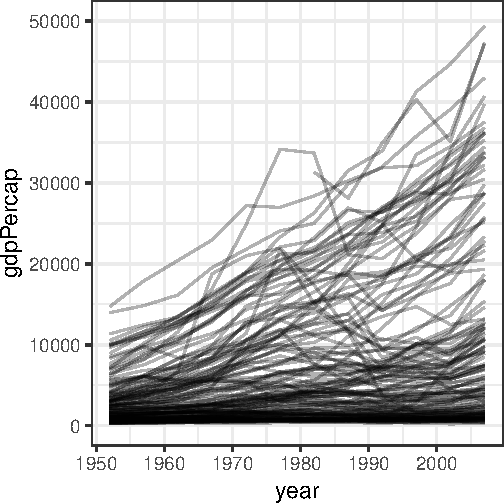
\includegraphics{Intro_tips_tricks_files/figure-latex/nest_mult_mod-1} \end{center}

Overall, it looks like GDP per capita has been steadily improving though
some countries see some declines.

\subsection{Nested data frame}\label{nested-data-frame}

This is best understood by means of examples.

\begin{Shaded}
\begin{Highlighting}[]
\KeywordTok{head}\NormalTok{(gapminder)}
\end{Highlighting}
\end{Shaded}

\begin{verbatim}
## # A tibble: 6 x 6
##   country     continent  year lifeExp      pop gdpPercap
##   <fct>       <fct>     <int>   <dbl>    <int>     <dbl>
## 1 Afghanistan Asia       1952    28.8  8425333      779.
## 2 Afghanistan Asia       1957    30.3  9240934      821.
## 3 Afghanistan Asia       1962    32.0 10267083      853.
## 4 Afghanistan Asia       1967    34.0 11537966      836.
## 5 Afghanistan Asia       1972    36.1 13079460      740.
## 6 Afghanistan Asia       1977    38.4 14880372      786.
\end{verbatim}

\begin{Shaded}
\begin{Highlighting}[]
\CommentTok{# What nesting does}
\NormalTok{nest_country <-}\StringTok{ }\NormalTok{gapminder }\OperatorTok
\StringTok{  }\NormalTok{dplyr}\OperatorTok{::}\KeywordTok{group_by}\NormalTok{(country, continent) }\OperatorTok
\StringTok{  }\NormalTok{tidyr}\OperatorTok{::}\KeywordTok{nest}\NormalTok{()}

\NormalTok{nest_country}
\end{Highlighting}
\end{Shaded}

\begin{verbatim}
## # A tibble: 142 x 3
##    country     continent data             
##    <fct>       <fct>     <list>           
##  1 Afghanistan Asia      <tibble [12 x 4]>
##  2 Albania     Europe    <tibble [12 x 4]>
##  3 Algeria     Africa    <tibble [12 x 4]>
##  4 Angola      Africa    <tibble [12 x 4]>
##  5 Argentina   Americas  <tibble [12 x 4]>
##  6 Australia   Oceania   <tibble [12 x 4]>
##  7 Austria     Europe    <tibble [12 x 4]>
##  8 Bahrain     Asia      <tibble [12 x 4]>
##  9 Bangladesh  Asia      <tibble [12 x 4]>
## 10 Belgium     Europe    <tibble [12 x 4]>
## # ... with 132 more rows
\end{verbatim}

\begin{Shaded}
\begin{Highlighting}[]
\CommentTok{# Accessing country-level data}
\NormalTok{nest_country}\OperatorTok{$}\NormalTok{data[[}\DecValTok{1}\NormalTok{]] }\CommentTok{#Afghanistan}
\end{Highlighting}
\end{Shaded}

\begin{verbatim}
## # A tibble: 12 x 4
##     year lifeExp      pop gdpPercap
##    <int>   <dbl>    <int>     <dbl>
##  1  1952    28.8  8425333      779.
##  2  1957    30.3  9240934      821.
##  3  1962    32.0 10267083      853.
##  4  1967    34.0 11537966      836.
##  5  1972    36.1 13079460      740.
##  6  1977    38.4 14880372      786.
##  7  1982    39.9 12881816      978.
##  8  1987    40.8 13867957      852.
##  9  1992    41.7 16317921      649.
## 10  1997    41.8 22227415      635.
## 11  2002    42.1 25268405      727.
## 12  2007    43.8 31889923      975.
\end{verbatim}

Now we apply previously discussed ideas from functional programming to
such nested dataframes. We want to check if the trend has been rising
for each country. This can be achieved by applying a trend-computing
function to each dataframe in the nested object.

\begin{Shaded}
\begin{Highlighting}[]
\CommentTok{# Trend computing function for GDP per capita}
\NormalTok{lm_gdppc_year <-}\StringTok{ }\ControlFlowTok{function}\NormalTok{(data_frame)}
\NormalTok{\{}
\NormalTok{  temp <-}\StringTok{ }\KeywordTok{lm}\NormalTok{(}\DataTypeTok{data =}\NormalTok{ data_frame,}
             \DataTypeTok{formula =}\NormalTok{ gdpPercap }\OperatorTok{~}\StringTok{ }\NormalTok{year) }\CommentTok{#trend}
  \KeywordTok{return}\NormalTok{((temp))}
\NormalTok{\}}

\CommentTok{# Update the nested dataframe by incorporating trends}
\NormalTok{nest_country <-}\StringTok{ }\NormalTok{nest_country }\OperatorTok
\StringTok{  }\NormalTok{dplyr}\OperatorTok{::}\KeywordTok{mutate}\NormalTok{(}\DataTypeTok{trend =} \KeywordTok{map}\NormalTok{(data, lm_gdppc_year))}
\CommentTok{# Equivalently: map(nest_country$data, lm_gdppc_year)}

\NormalTok{nest_country}\OperatorTok{$}\NormalTok{trend[[}\DecValTok{1}\NormalTok{]] }\CommentTok{#Afghanistan}
\end{Highlighting}
\end{Shaded}

\begin{verbatim}
## 
## Call:
## lm(formula = gdpPercap ~ year, data = data_frame)
## 
## Coefficients:
## (Intercept)         year  
##   1674.8134      -0.4406
\end{verbatim}

\begin{Shaded}
\begin{Highlighting}[]
\CommentTok{# We can also do the standard procedures}
\NormalTok{nest_country }\OperatorTok
\StringTok{  }\NormalTok{dplyr}\OperatorTok{::}\KeywordTok{filter}\NormalTok{(continent }\OperatorTok{==}\StringTok{ 'Asia'}\NormalTok{)}
\end{Highlighting}
\end{Shaded}

\begin{verbatim}
## # A tibble: 33 x 4
##    country          continent data              trend 
##    <fct>            <fct>     <list>            <list>
##  1 Afghanistan      Asia      <tibble [12 x 4]> <lm>  
##  2 Bahrain          Asia      <tibble [12 x 4]> <lm>  
##  3 Bangladesh       Asia      <tibble [12 x 4]> <lm>  
##  4 Cambodia         Asia      <tibble [12 x 4]> <lm>  
##  5 China            Asia      <tibble [12 x 4]> <lm>  
##  6 Hong Kong, China Asia      <tibble [12 x 4]> <lm>  
##  7 India            Asia      <tibble [12 x 4]> <lm>  
##  8 Indonesia        Asia      <tibble [12 x 4]> <lm>  
##  9 Iran             Asia      <tibble [12 x 4]> <lm>  
## 10 Iraq             Asia      <tibble [12 x 4]> <lm>  
## # ... with 23 more rows
\end{verbatim}

\subsubsection{Unnesting}\label{unnesting}

The \texttt{unnest()} function undoes the nesting:

\begin{Shaded}
\begin{Highlighting}[]
\NormalTok{tidyr}\OperatorTok{::}\KeywordTok{unnest}\NormalTok{(nest_country, data)}
\end{Highlighting}
\end{Shaded}

\begin{verbatim}
## # A tibble: 1,704 x 6
##    country     continent  year lifeExp      pop gdpPercap
##    <fct>       <fct>     <int>   <dbl>    <int>     <dbl>
##  1 Afghanistan Asia       1952    28.8  8425333      779.
##  2 Afghanistan Asia       1957    30.3  9240934      821.
##  3 Afghanistan Asia       1962    32.0 10267083      853.
##  4 Afghanistan Asia       1967    34.0 11537966      836.
##  5 Afghanistan Asia       1972    36.1 13079460      740.
##  6 Afghanistan Asia       1977    38.4 14880372      786.
##  7 Afghanistan Asia       1982    39.9 12881816      978.
##  8 Afghanistan Asia       1987    40.8 13867957      852.
##  9 Afghanistan Asia       1992    41.7 16317921      649.
## 10 Afghanistan Asia       1997    41.8 22227415      635.
## # ... with 1,694 more rows
\end{verbatim}

\subsubsection{Evaluating model fits}\label{evaluating-model-fits}

The \texttt{glance()} function from the package \texttt{broom} (included
in \texttt{tidyverse}) is useful

\begin{Shaded}
\begin{Highlighting}[]
\NormalTok{nest_country }\OperatorTok
\StringTok{  }\NormalTok{dplyr}\OperatorTok{::}\KeywordTok{mutate}\NormalTok{(}\DataTypeTok{model_fit =} \KeywordTok{map}\NormalTok{(trend, broom}\OperatorTok{::}\NormalTok{glance)) }\OperatorTok
\StringTok{  }\NormalTok{tidyr}\OperatorTok{::}\KeywordTok{unnest}\NormalTok{(model_fit)}
\end{Highlighting}
\end{Shaded}

\begin{verbatim}
## # A tibble: 142 x 15
##    country continent data  trend r.squared adj.r.squared sigma statistic
##    <fct>   <fct>     <lis> <lis>     <dbl>         <dbl> <dbl>     <dbl>
##  1 Afghan~ Asia      <tib~ <lm>    0.00539       -0.0941  113.    0.0542
##  2 Albania Europe    <tib~ <lm>    0.678          0.646   710.   21.1   
##  3 Algeria Africa    <tib~ <lm>    0.782          0.760   641.   35.9   
##  4 Angola  Africa    <tib~ <lm>    0.129          0.0422 1141.    1.48  
##  5 Argent~ Americas  <tib~ <lm>    0.706          0.677  1059.   24.0   
##  6 Austra~ Oceania   <tib~ <lm>    0.969          0.966  1432.  318.    
##  7 Austria Europe    <tib~ <lm>    0.996          0.996   620. 2654.    
##  8 Bahrain Asia      <tib~ <lm>    0.866          0.852  2081.   64.5   
##  9 Bangla~ Asia      <tib~ <lm>    0.649          0.614   146.   18.5   
## 10 Belgium Europe    <tib~ <lm>    0.993          0.992   728. 1453.    
## # ... with 132 more rows, and 7 more variables: p.value <dbl>, df <int>,
## #   logLik <dbl>, AIC <dbl>, BIC <dbl>, deviance <dbl>, df.residual <int>
\end{verbatim}


\end{document}
